\begin{figure}[t]
  \centering
  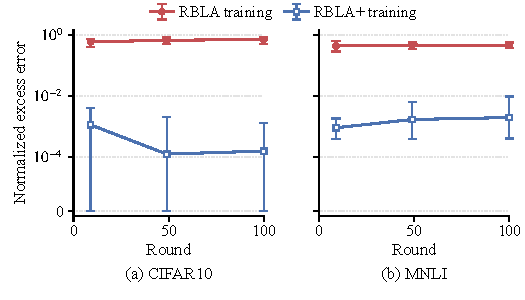
\includegraphics[width=\columnwidth]{rbla+/figures/ablation/figure_3_prefix_quality/prefix_reconstruction_quality.pdf}
  \caption{CIFAR10 and MNLI. Raw-prefix quality along the two training paths. Markers and bars show the median and interquartile range of $(\|X-X_{\mathrm{prefix},q}\|_F^2-\|X-X_{\mathrm{dense},q}\|_F^2)/\|X\|_F^2$ over all layer/unique-width pairs with $q<Q$ within each checkpoint. Bars are not seed confidence intervals. The horizontal axis spans rounds 0--100; measured checkpoints are logged rounds 9, 49 and 100. The symmetric-logarithmic vertical scale is linear below $10^{-5}$. Reference aggregates differ across paths; RBLA+ includes bidirectional RankScale.}
  \label{fig:ablation-prefix-quality}
\end{figure}
